\Chapter{Generálás}
\Section{Úthálózat Generálása}
Maga a generáló algoritmus megalkotásakor első lépésben a nagyvonalakban leírt elvárt működést vizsgáltam. A hálózatnak középponttól kifelé haladva ritkulnia kell, ezzel közelítve egy 
valódi várost. A paraméterezéssel kapcsolatos elvárásokat könnyen meg lehet valósítani. Egy gráfként képzelhető el a megalkotott úthálózat, melynek csomópontjai jelölik az egyes útelemek 
elejét, élei pedig azoknak tartományát. A gráf 0. szintjét jelöltem el a hálózat középpontjának, innen mindig 4 irányba indulnak élek. Mivel az egy csomópontból kiinduló maximális élek számának 4-et választottam,
 ez garantálja hogy a középpontnak kijelölt ponttól minden irányba nagyjából egyenletes mértékben terjedjen az úthálózat. Minden további csomópont generálódásakor kapja meg 
annak értékét, hogy mennyi irányba indulnak belőle élek. 
\subsection{Generáló algoritmus}
A csomópontok generálása a következőképpen történik:
\begin{enumerate}
\item A kiválasztott csomópont kap egy véletlenszerű irányt, észak, dél, kelet, vagy nyugat értékében
\item Ha a kapott érték megegyezik azzal az iránnyal amerre a csomópont szülője van, vagy már indult arra belőle él, újat kap
\item A kiválasztott iránynak megfelelő véletlen generált X és Y koordinátákat kap
\item A kapott koordinátákból alkotott csomópont felkerül a gráfra
\item Ha a jelenlegi csomópontból még kell éleket indítani, akkor kezdődik előröl
\end{enumerate}
Az előbbiekben említett X és Y koordinátát kissé pontosítanám. Ha a csomópontot nyugat vagy kelet irányba generáljuk, az X koordináta értéke a jelenlegi pont X koordinátája, hozzáadva egy
előre definiált értékek közötti véletlen szám. Az Y koordináta ilyenkor egy minimális eltérés az út fekvésében, hasonlóan generálódik, de lényegesen alacsonabb véletlen számot kap. Ez
tulajdonképpen a valóságban is látható "tökéletlenségekre" vezethető vissza, ugyanis a legtöbb esetben ott sem teljesen merőleges egymásra kettő út. Az észak és dél irányba induló pontok 
esetén ugyan ez az eljárás, csak a két koordináta szerepe felcserélődik.
Fontos viszont az is, hogy a középponttól távolodva átlagosan kevesebb elágazása legyen egy csomópontnak, ezért ehhez felhasználható annak gráfbeli szintje. Minden csomópontról eltárolódik 
annak szintje (szülő szintje + 1), ami befolyásolja az elágazások számát. Egy másik probléma az, hogy az így generált élek gyakran metszhetik egymást, amely az aluljárók és a hídak hiányában 
itt nem megengedett, ezért utolsó lépésnek ellenőrizni kell hogy az új él metszi-e bármely meglévő élek közül akár az egyiket is, és ha igen akkor nem kerülhet fel a gráfra. Az él viszont hozzáadható 
az eredetileg kijelölt csomóponthoz legközelebbi csomóponttal történő helyettesítéssel, feltéve ha így nem történik létező út metszése.
A buszmegállók elhelyezésével kapcsolatban a következő feltételeket
adtam:
\begin{itemize}
\item A legcélszerűbb a hálózat két, egymástól távol lévő, a gráf mélyebb szintjein elhelyezkedő pont közötti út létrehozása
\item Az útvonalnak érintenie kell a középpontot, a gráf 0. szintjét
\item Lehető legkevesebbszer érintse többször ugyan azt a csomópontot
\end{itemize}
Ennek érdekében először kijelölöm az út egyik végét, mint megállót. Ezek után keresek egy utat a gráf 0. szintjéhez, melyen legfeljebb minden második csomópontot kijelölöm megállónak. A középpont 
elérése után kijelölöm a második végpontot, mely a középponttól az eddigi iránynak ellentétesen, a gráf mélyebb szintjei közül kell lennie. Az ehhez a középpontból vezető úton, az utóbbihoz hasonló 
eljárással kijelölök megállókat. Az utak sávszámának meghatározására a gráfbeli mélységüket használom. A magasabb szinten lévő élek nagyobb valószínűséggel lesznek többsávosak. Ez a generálás végén választódik
ki. Az egyirányú utak kijelölése is a folyamat legvégén történik. Ennek az oka magából az utak jellegéből adódik, ugyanis egyirányú út nem végződhet zsákutcában, és nem is zárhatja el a hálózat egy részét a többi elől. Éppen ezért egy olyan részgráfot kell találni amely Hamilton-kört alkot, amelyen egy részgráfot már nyugodtan egyirányúvá lehet tenni.
\subsection{Az egyirányú út}
Egy könnyű módszer annak megoldására, hogy mely utak lehetnek egyirányúak az lenne, ha a generálás során egymást metszett utakból kialakult éleket jelölöm el egyirányúnak. Ezek az élek ugyanis biztos hogy egy létező Hamilton-út részei, mivel az eredetileg fagráfnak megfelelő úthálózat bármely két csomópontja közé húzott él Hamilton-utat ad.
\Section{Alapelemek megjelenítése HTML Canvas segítségével}
\subsection{Fejlesztői környezet felállítása}
Az algoritmus működését, eredményét egy HTML Canvas objektumon szemléltetem. Magát a kódot JavaScript-ben írtam, annak ECMAScript 6-os verziójában. Fejlesztői környezetnek A JetBrains által készített WebStormot használtam. Először is 
létrehoztam egy HTML fájlt, ahol a body tag-en belül elhelyeztem a canvas elemet. Erre az elemre JavaScriptből a HTML-ben megadott id-je alapján lehet hivatkozni. Ezután létrehoztam egy JavaScript fájlt, melyben egy (document).ready() szintaktikában 
elhelyezett függvényhívással indítom a generálást. A (document).ready() a jQuery függvénykönyvtárnak része. Azért szükséges ebben az esetben, mert ameddig a html fájl nem töltött be teljesen, a script nem futtatható mert a canvas elemre nem létezne 
semmilyen referencia. Ez a részlet biztosítja hogy csak akkor kezdődjön a script futtatása, ha a HTML documentum teljesen betöltött. 
\subsection{Létrehozott osztályok}
\subsubsection{Node}
A gráfon egy csomópontot leíró objektum. Egy konstruktort tartalmaz, amely beállítja az osztály 6 adattagjának értéket. Ezek az adattagok a következőek:
\begin{itemize}
\item x: A csomópont X koordinátája
\item y: A csomópont Y koordinátája
\item branches: Hányfelé kell tovább ágaztatni a csomópontot
\item level: A gráf hanyadik szintjén helyezkedik el a csomópont
\item connectedFrom: Milyen irányból lett kiterjesztve a csomópont
\item parentNodeIndex: A gráfban lévő csomópontokat tartalmazó vektoron belül ezen csomópont szülőjének indexe
\end{itemize}
\subsubsection{Edge}
A gráfon egy él leírására szolgáló objektum. Egy konstruktort tartalmaz, amely inicializálja 4 adattagját. Ezek az alábbiak:
\begin{itemize}
\item from: Az a csomópont, ahonnan az él kezdődik
\item to: Az a csomópont, amiben az él végződik
\item lanes: Az él által jelölt úton hány sáv van
\item oneway: Logikai változó, az út egyirányú-e vagy sem
\end{itemize}
\subsubsection{Graph}
Magát a gráfot leíró objektum, mely tartalmaz 2 függvényt annak canvas-on történő kirajzolására. Paraméter nélküli konstruktora 2 adattagját inicializálja üres értékkel. Adattagjai és függvényei a következők:
\begin{itemize}
\item Nodes: A csomópontokat tartalmazó vektor
\item Edges: Az éleket tartalmazó vektor
\item drawAllNodes: Függvény, mely végig iterál a Nodes vektoron, és mindegyik elemére meghívja a kirajzoló függvényt
\item drawAllEdges: Függvény, végig iterál az Edges vektoron, egyirányú út esetén nyilat rajzol, ellenkező esetben egyenes vonalat
\end{itemize}
\subsection{Segédfüggvények}
\subsubsection{intersects}
Ez a függvény arra szolgál, hogy kiszámítsa két él metszi-e egymást. Ehhez két paramétert vár, edge1 és edge2 néven. Visszatérési értéke logikai típusú.
\subsubsection{distance}
Két csomópont közötti távolság kiszámítására szolgáló függvény. Ehhez a két vektor által meghatározott szakasz hosszát számolja ki pitagorasz tétellel. Ezzel az eredménnyel tér vissza.
\subsubsection{maxBranchesReached}
Ezzel a függvénnyel megmondható hogy egy adott csomópontba már lett-e 4 él húzva. A függvény paramétereiként megkapja a keresett csomópontot, a gráfot, és a jelenleg kiterjesztés alatt álló csomópont gráfbeli indexét. Amennyiben a gráfban megtalált csomópont branches értéke kisebb mint 3, akkor növeli 1-el és hamis értékkel tér vissza, azaz még nem volt 4 él húzva. Ellenkező esetben igaz értéket ad.
\subsubsection{getBranchCount}
Ez a függvény egy egész számot kap paraméterként, mely egy csomópont gráfbeli mélységére utal. Ez alapján a szám szerint visszaadja hogy mennyi irányba ágazzon el az adott csomópont. Első szinten 80\% az esélye hogy 4 irányban ágazik el, ez szintenként 20\%-al csökken. Ha nem 4 irányban ágazik el, véletlenszerűen generált számot ad vissza 0 és 2 között, mivel a csomópont szülőjéhez vezető élt ilyenkor nem számoljuk.
\subsubsection{findMaxLevelNodes}
A gráf legmélyebb szintjén lévő csomópontok megtalálására szolgáló függvény. Paraméterként megkapja a gráfot. Első lépésben beállítja a max értéket a gráf első csomópontjának szintjére, és inicializálja a maximális mélységben elhelyezkedő csomópontok vektorát. Ezután maximum kereséssel beállítja max értéket. Majd a gráf Nodes vektorán végig iterálva hozzáadja az ezen max értéknek megfelelő mélységű csomópontokat az eredmény vektorhoz. Végül ezzel a vektorral tér vissza.
\subsubsection{DrawBStops}
Buszmegálló rajzolására használt függvény. Egy csomópontot kap paraméterként. A kontextust felhasználva felrajzolja a canvasra egy zöld négyzet formájában. Visszatérési értéke nincs.
\subsubsection{makeBusStops}
Ez a függvény szolgál a buszmegállók elhelyezésére. Egyelőre csak a hozzávetőleges helyüket jelöli, nem az él közepére teszi a helyüket, hanem a csomópontokra. Paraméterként megkapja a gráfot. Előszőr meghívja a findMaxLevelNodes függvényt, ebből a kapott értéket eltárolja egy változóba. 

Kijelöl az útvonal kezdetének az előbb kapott vektorból egy véletlenszerű elemet. Ezt felrajzolja a DrawBStops függvénnyel. Ezután végig iterál a maximum mélységű tömbökön, maximum keresést végezve a kiindulási ponttól mért távolságot illetően. Ehhez a distance függvényt használja. Ha megvan a végpont azt is felrajzolja. 
Ezután elindul a kiindulási ponttól, sorra véve a csomópontok szüleit. Minden buszmegálló kirajzolása után kap egy véletlen értéket, amely megmondja hogy hány csomópont után kell rajzolnia mégegyet. Ha eljutott a gráf kezdőpontjáig megcsinálja ugyan ezt az út végpontjától is. Visszatérési értéke nincs.
\subsubsection{drawCanvasNode}
Egy paraméterként megkapott csomópont koordinátáinak megfelelő helyre négyzetet rajzol a canvasre.
\subsubsection{drawCanvasEdge}
Egy élt kap meg paraméterként, melynek kezdő és végpontjai között egyenes vonalat húz a canvasre.
\subsection{A generáló függvény}
Ha ez megtörtént, meghívódik a DrawOnCanvas függvény. Először is ez eltárolja változóként a canvas-ra vonatkozó referenciát.
szintén új változóba, utána a myCanvas.getContext("2d") létrehoz egy CanvasRenderingContext2D objektumot, mellyel a canvasra rajzolni lehet. A következő lépésben megtörténik a paraméterek beállítása, azaz mennyi legyen a maximális csomópontok száma, átlagosan milyen hosszúak legyenek az utak. 
A kontextust elmozdítjuk alapértelmezett helyéről, (0,0)-ról az (1000,500) pontba. Létrehozzuk a kezdő csomópontot ezen a pozíción%, és hozzáadjuk a csomópontokat tartalmazó tömbhöz. Létrehozzuk az éleket tartalmazó tömböt, majd kirajzoljuk az első csomópontot, melyet egy négyzettel ábrázolok a kontextus .fillRect() függvényével. 
%A többi csomópont generálásához itt egy ciklust indítok, mely addig fog futni ameddig a csomópontokat tartalmazó tömb elemszáma el nem éri a paraméterként megadott értéket. Minden iterációban a csomópontok tömbjéből a következő elemet választja ki első lépésben, a 0-tól indulva. 
%A kontextust áthelyezem a jelenlegi csomópont pozíciójába, majd beállítok négy logikai változót, melyek megadják hogy ebből a csomópontból a négy irány közül valamelyikébe mentünk-e már tovább. Kezdetben mindegyik hamis értéket kap. Ezt követően egy switch utasítással megkeresem melyik az az irány ahonnan az adott 
%csomópontot kiterjesztettük, és ennek megfelelően arra nem mehet tovább. Akár úgy is lehet venni hogy a jelenlegi pontból arrafelé már "húztunk élet", a logikai változó értéke erre vonatkozóan hamissá válik. Különleges eset a kiindulási pont viszont, 
%ahol egyik irányra sem igaz ez, ezért csak szimplán továbbmegy a program. Ezután következik egy újabb ciklus, mely a csomópontból húzandó éleken iterál végig, tehát a kiindulási pontnál 4 alkalommal fog ismétlődni. Legelőször is belép egy végtelen ciklusba, %ahonnan csak akkor szabadulhat 
%break utasítással, ha a ciklus elején véletlenszerűen kisorsolt irányba húzható él. Ha nem akkor újat sorsol. Ezután egy switch szerkezet következik a direction nevű változóra, mely az előbb kapott irányt tárolja. Észak és dél esetén az új csomópont X %koordinátája egy 
%előre definiált (minimális) értékek közötti véletlen szám, melyhez hozzáadjuk a jelenlegi pont X koordinátáját. Ez a szám negatív is lehet. Az Y koordináta kiszámításánál is hasonló a helyzet, de itt nagyobb számokat várunk, amelyek csak pozitívak lehetnek. Ha észak felé terjeszkedünk, 
%a kapott véletlen számot beszorozzuk -1-el, ehhez hozzáadva a kiindulási Y értéket, megkapjuk az új pont koordinátáját. Nyugat és Kelet esetében annyi a különbség, hogy a két koordináta generálásában az eljárás felcserélt.
%Ezek után gráf mélységének függvényében generálódik egy szám, amely megadja hogy az új csomópont hányfelé fog szétágazni. Annak az esélye hogy négyfelé ágazik kezdetben 100\%, majd minden egyes mélységi szinttel 20\%-al csökken, végül 20\% esélynél megáll. 
%Ha egy csomópont nem teljes, azaz 4-felé ágazó, akkor véletlenszerűen adódik hogy 2, vagy 3 ágú. Ez után beállítunk egy invalidedge nevű logikai változó hamis értékre, és elkezdjük végigiterálni egy újabb ciklusban az eddig létező élek tömbjét.
%Ha még nem léteznek élek, azaz ez az első él generálása, ezt a részt átugorja. Ellenkező esetben minden élre meghívódik egy külön függvény intersects néven. Ennek a függvénynek argumentumaiként meg kell adni mindkét él két végpontjának az x és y koordinátáit, azaz 
%összesen 8 argumentumot. Ez a függvény igaz értéket ad vissza ha a két szakasznak van közös pontja. Működésének alapja az ezen pontok által kapott két egyenes feltételezett közös pontjára vonatkozó egyenletrendszer. Ezen egyenletrendszer mátrixának a determinánsát nézi meg elsősorban. Ha ez 0, nem létezik a metszéspont. 
%Ha nem 0, akkor tudnunk kell hogy a metszéspont a szakaszokon van-e. Az egyenletből kapott lambda és gamma értékeknek egyaránt 0 és 1 közé kell esnie, ha a pont a két szakasz közé esik. Ha ez teljesül igaz értéket, ha nem akkor hamis értéket ad vissza a függvény. 
%Abban az esetben ha a kapott él metszett más élt, a végpontját áthelyezzük a hozzá legközelebbi csomópontra, viszont ha így is metszi az egyik másik élt, akkor elvetjük. Ha nem metszette semelyik élt, akkor Nodes.push()-al hozzáadjuk a tömbhöz az új pontot, felrajzoljuk a 
%canvas-ra, az Edges tömbhöz szintén hozzáadjuk a hozzá vezető élt, majd a kontextusnak a .lineto() és .stroke() metódusával felrajzoljuk a canvas-ra.
%Ezen alap eljárással a következő képhez hasonló eredményhez jutunk:

\begin{figure}[H]
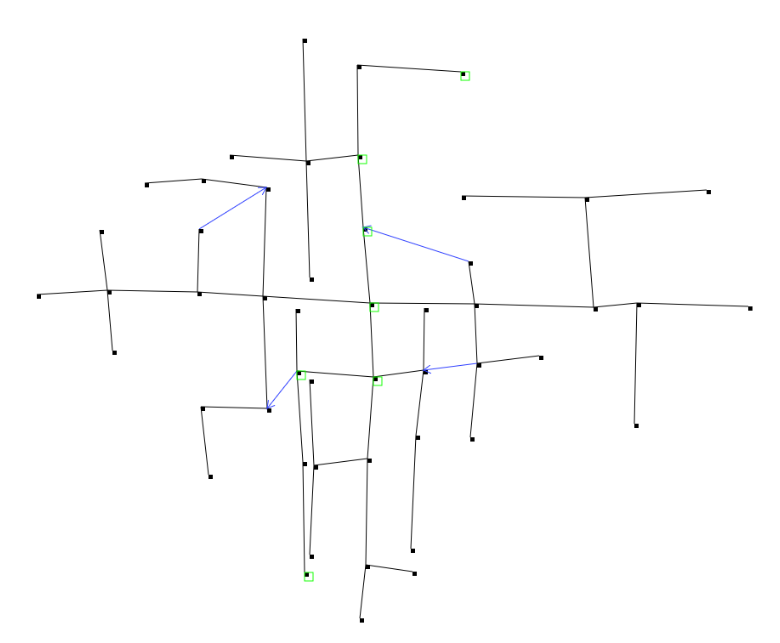
\includegraphics[width=\linewidth]{graph.png}
\caption{Kép a generáló algoritmus eddigi eredményéről}
\label{fig:graph}
\end{figure}
Ezek után következik az utak sávszámának kiadása, az egyirányú utak elhelyezése, valamint a buszmegállók generálása.